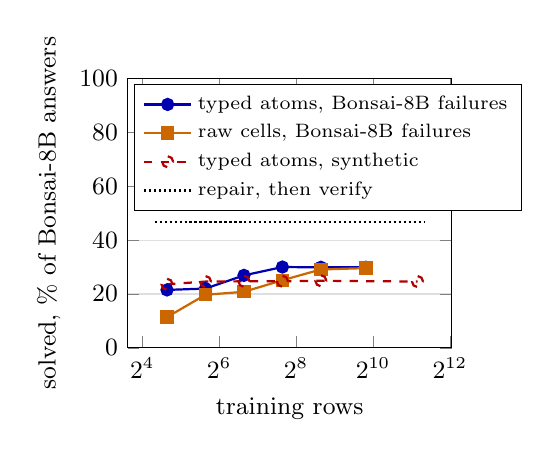
\begin{tikzpicture}
\begin{axis}[width=0.47\linewidth, height=5.0cm, xmode=log, log basis x=2, xlabel={training rows}, ylabel={solved, \% of Bonsai-8B answers},
  ymin=0, ymax=100, ymajorgrids, grid style={gray!25}, legend style={font=\scriptsize, at={(0.02,0.98)}, anchor=north west}, legend cell align=left,
  tick label style={font=\small}, label style={font=\small}]
\addplot[blue!70!black, mark=*, thick] coordinates {(25,21.5) (50,22.0) (100,26.9) (200,30.0) (400,29.9) (900,29.9)};
\addlegendentry{typed atoms, Bonsai-8B failures}
\addplot[orange!80!black, mark=square*, thick] coordinates {(25,11.4) (50,19.7) (100,20.8) (200,25.1) (400,29.1) (900,29.6)};
\addlegendentry{raw cells, Bonsai-8B failures}
\addplot[red!70!black, dashed, mark=o, thick] coordinates {(25,23.6) (50,24.6) (100,24.7) (200,24.7) (400,24.9) (2282,24.6)};
\addlegendentry{typed atoms, synthetic}
\addplot[black, densely dotted, thick, domain=20:2600, samples=2] {46.6};
\addlegendentry{repair, then verify}
\end{axis}
\end{tikzpicture}
